\documentclass[11pt]{article}

\usepackage{fullpage}
\usepackage{graphicx}
\usepackage{amsmath}
\usepackage{amssymb}
\usepackage{amsthm}
\usepackage{fancyvrb}

\parindent0in
\pagestyle{plain}
\thispagestyle{plain}

\newcommand{\myname}{Mehshan Mustafa}
\newcommand{\dated}{\today}

\newenvironment{theorem}[2][Theorem]{\begin{trivlist}
\item[\hskip \labelsep {\bfseries #1}\hskip \labelsep {\bfseries #2.}]}{\end{trivlist}}
\newenvironment{lemma}[2][Lemma]{\begin{trivlist}
\item[\hskip \labelsep {\bfseries #1}\hskip \labelsep {\bfseries #2.}]}{\end{trivlist}}
\newenvironment{exercise}[2][Exercise]{\begin{trivlist}
\item[\hskip \labelsep {\bfseries #1}\hskip \labelsep {\bfseries #2.}]}{\end{trivlist}}
\newenvironment{problem}[2][Problem]{\begin{trivlist}
\item[\hskip \labelsep {\bfseries #1}\hskip \labelsep {\bfseries #2.}]}{\end{trivlist}}
\newenvironment{question}[2][Question]{\begin{trivlist}
\item[\hskip \labelsep {\bfseries #1}\hskip \labelsep {\bfseries #2.}]}{\end{trivlist}}
\newenvironment{corollary}[2][Corollary]{\begin{trivlist}
\item[\hskip \labelsep {\bfseries #1}\hskip \labelsep {\bfseries #2.}]}{\end{trivlist}}
\newenvironment{solution}{\begin{proof}[Solution]}{\end{proof}}
\newenvironment{idea}[2][Proof Idea.]{\textit{#1} #2}

\begin{document}
\textbf{Introduction to the Theory of
Computation}\hfill\textbf{\myname}\\[0.01in]
\textbf{Chapter 1: Reqular Languages}\hfill\textbf{\dated}\\
\smallskip\hrule\bigskip

\begin{problem}{1.40}
Recall that string $x$ is a \textbf{prefix} of string $y$ if a string $z$ exists where $xz = y$, and that $x$ is a proper prefix of $y$ if in addition $x \neq y$. In each of the following parts, we define an operation on a language A. Show that the class of regular languages is closed under that operation.
\end{problem}

\begin{problem}[Part]{a}
$NOPREFIX(A) = \{ w \in A \ | \ no \ proper \ prefix \ of \ w \ is \ a \ member \ of \ A \}.$
\end{problem}

\begin{idea}
Let the regular expression $R=0^{*}10^{*}$ describe the language $A$.
\[ A = \{ 1, 01, 10, 010, 001, \cdots \} \]
\[ NOPREFIX(A) = \{ 1, 01, 001, \cdots \} \]
\begin{center}
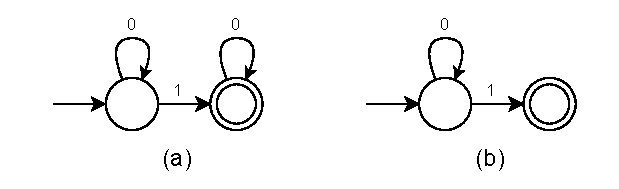
\includegraphics[scale=1.0]{Figures/Problem1.40a.pdf} \\
State diagrams of finite automata that recognize $A$ (a) and $NOPREFIX(A)$ (b). Take the finite automaton that recognizes $A$, and remove all transitions from accept states to any other state to construct the finite automaton to recognize $NOPREFIX(A)$.
\end{center}\end{idea} 

\begin{proof}
The proof is by construction. Let $N = (Q, \Sigma, \delta, q_{0}, F)$ be the DFA that recognizes $A$. Construct the NFA $N' = (Q', \Sigma, \delta', q_{0}', F')$ to recognize $NOPREFIX(A)$:
\begin{enumerate}
\item $Q' = Q$
\item $q_{0}' = q_{0}$
\item $F' = F$
\item Define $\delta'$(q, a) so that for any $q \in Q'$ and any $a \in \Sigma$:
\end{enumerate}
\begin{center}
$\displaystyle \delta'( q,\ a) \ =\begin{cases}
\{ \delta( q,\ a) \} & q \notin F \\
\phi & q \in F \\
\end{cases} \ \ $
\end{center}
\end{proof}

\newpage 

\begin{problem}[Part]{b}
$NOEXTEND(A) = \{ w \in A \ | \ w \ is \ not \ the \ proper \ prefix \ of \ any \ string \ in \ A \}.$
\end{problem}

\begin{idea}
Let $A = \{ aa, aab \}$, then $NOEXTEND(A) = \{ aab \}$
\begin{center}
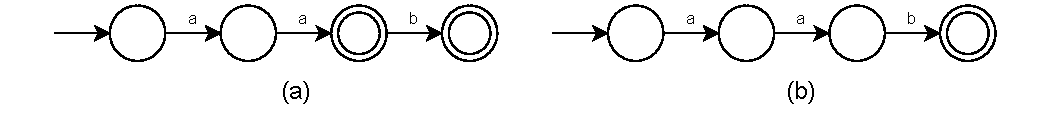
\includegraphics[scale=0.8]{Figures/Problem1.40b.pdf} \\
State diagrams of finite automata that recognize $A$ (a) and $NOEXTEND(A)$ (b). Take the finite automaton that recognizes $A$, and change any accept state $q$ into non-accept state, if there exists a sequence of transitions from $q$ to any accept state (including $q$ itself).
\end{center}\end{idea}

\begin{proof}
The proof is by construction. Let $N = (Q, \Sigma, \delta, q_{0}, F)$ be the DFA that recognizes $A$. Construct the DFA $N' = (Q, \Sigma, \delta, q_{0}, F')$ to recognize $NOEXTEND(A)$:
\begin{enumerate}
\item $N'$ has the same states $Q$, start state $q_{0}$ and $\delta$ as $N$.
\item $F' = \{ q \ | \ q \in F \ and \ there \ is \ no \ sequence \ of \ transitions \ from \ q \ to \ any \ accept \ state \ \}$
\end{enumerate}
\end{proof}
\end{document}